% Tento soubor nahraďte vlastním souborem s obsahem práce.
%=========================================================================
% Autoři: Michal Bidlo, Bohuslav Křena, Jaroslav Dytrych, Petr Veigend a Adam Herout 2019

% Pro kompilaci po částech (viz projekt.tex), nutno odkomentovat a upravit
%\documentclass[../projekt.tex]{subfiles}
%\begin{document}

\chapter{Úvod}
\label{uvod}
Data a informace dnes představují jeden z nejcennějších zdrojů moderní společnosti. Často jsou označována jako "digitální zlato", protože jejich správné 
využití může přinést obrovskou hodnotu v různých oblastech – od vědy a průmyslu až po zdravotnictví a každodenní život. Aby však mohla být efektivně využita, 
je nutné je správně zaznamenávat, ukládat a analyzovat.

Vzhledem k široké škále oblastí, kde data vznikají, se používají různé metody jejich sběru a uchovávání. Data mohou pocházet z různých zdrojů – například 
senzorů měřících fyzikální veličiny, síťových zařízení sledujících internetový provoz, medicínských přístrojů monitorujících životní funkce pacientů, 
ekonomických systémů analyzujících finanční transakce či průmyslových strojů zaznamenávajících provozní parametry. Každý z těchto zdrojů má specifické 
požadavky na způsob sběru, formátování a uchovávání dat. 

Tato bakalářská práce je věnována návrhu a implementaci takového zařízení, které bude schopno záznamu dat. Požadavek na zařízení vznikl od firmy NXP 
Semiconductors, konkrétně od týmu zaměřeného na bezdrátové nabíjení, ve kterém pracuji. Tento tým působí v České republice – v pobočkách v Brně a Rožnově 
pod Radhoštěm – a zároveň má své zastoupení v Asii a Severní Americe. NXP Semiconductors je jedním z předních členů WPC (Wireless Power Consortium), organizace 
zodpovědné za definování standardu Qi pro bezdrátové nabíjení. Primární zaměření NXP v této oblasti spočívá ve vývoji referenčních designů pro automotive 
sektor, kde zákazníkům poskytuje řešení určená pro integraci do vozidel.

Zákazníci, kteří využívají referenční designy NXP, pocházejí z celého světa a dostávají téměř hotový produkt, který lze následně certifikovat v Qi 
certifikačních laboratořích. Nicméně i přesto, že jsou referenční designy navrženy podle nejnovějších standardů, často dochází k jejich úpravám podle 
specifických požadavků zákazníků, zejména s ohledem na konkrétní poptávku koncového zákazníka (OEM – Original Equipment Manufacturer). Tyto požadavky 
jsou obvykle shrnuty v RFQ (Request for Quotation), kde zákazník specifikuje konkrétní požadavky na systém. Tyto úpravy mohou být například realizovány 
z důvodu snížení ceny nebo zlepšení výkonu, například EMC charakteristik a nebo speciální chování bezdrátové nabíječky v krajních situacích. 

Při jakýchkoli úpravách však vznikají nové technické výzvy, a proto NXP poskytuje zákazníkům plnou technickou podporu až do úspěšné certifikace. Certifikace 
probíhá v různých laboratořích po celém světě, avšak ne vždy může být přítomen zaměstnanec NXP, který by dohlížel na celý proces a zajistil, že certifikace 
proběhne hladce. V těchto případech se tým pro bezdrátové napájení spoléhá na záznamy poskytnuté operátorem certifikační laboratoře. Tyto záznamy však 
pocházejí pouze ze strany přijímače – tedy certifikačního zařízení, nejčastěji od výrobců Nok9 nebo Granite River Labs (GRL). Bohužel tyto údaje nezahrnují 
explicitní informace o chování vysílače a pokud tedy bezdrátová nabíječka - vysílač nějakým testem neprojde (což se občas stává), je často náročné zpětně 
identifikovat příčinu problému. \cite{nxp_wireless_charging_team}


\chapter{Záznam dat}
\label{zaznam_dat}

\section{Počátky záznamu a zpracování dat (Historie záznamu a zpracování dat - předchozí název)}
\label{historie}
Lidstvo, již od svých počátků potřebovalo zaznamenávat data, pomocí nich se totiž učilo z minulých zkušeností, předávalo znalosti dalším generacím, 
organizovalo společenské a obchodní procesy a zajišťovalo rozvoj vědy a technologií. Proto se již od pravěku hledaly způsoby, jak evidovat důležité 
události a hodnoty. První formy záznamu dat sahají až 19 000 let před Kristem, kdy v paleolitu vznikl nástroj známý jako kost Ishango. Tento jednoduchý 
nástroj, vyrobený z kosti paviána, obsahoval vyryté zářezy, které pravděpodobně sloužily k provádění základních matematických operací, jako je sčítání či 
násobení.

\begin{figure}[h] % obrazek ishango
    \centering
    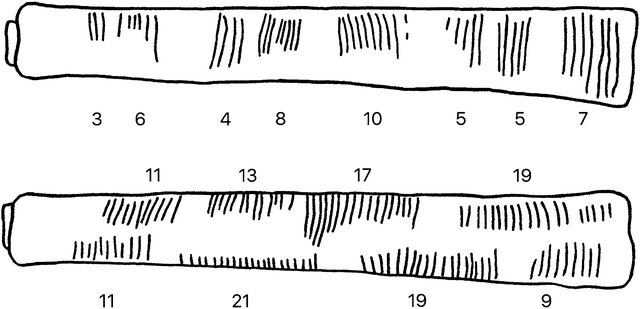
\includegraphics[width=0.6\textwidth]{obrazky-figures/ishango.jpg}
    \caption{Kost Ishango sloužící k záznamu informací v době Paleolitu \cite{ishango_picture}}
    \label{fig:ishango}
\end{figure}

S příchodem prvních civilizací se začaly vyvíjet lepší metody uchovávání dat. Ve starověké Mezopotámii, oblasti mezi Eufratem a Tigridem, kde sídlil národ 
Sumérů, vzniklo kolem roku 3400 před naším letopočtem klínové písmo. Tento typ písma byl využíván hlavně pro zápis obchodních transakcí, zákonů a dalších 
důležitých informací, které byly zaznamenávány na hliněné tabulky pomocí rákosového stylusu. O několik století později, kolem roku 3200 př. n. l., začali 
Egypťané používat hieroglyfy, které byly ryty do kamene nebo zapisovány na papyrus, což umožnilo uchovávat důležité administrativní a náboženské záznamy. 
V Číně se mezi 1200–1000 př. n. l. používaly věštecké kosti, na které se zaznamenávaly otázky kladené orákulu - což jsou důležité otázky, zejména ve věcech 
budoucnosti, i jeho odpovědi, čímž vznikly první organizované záznamy psané ranými čínskými znaky.

\newpage

Průlomem pro zaznamenáváním dat, bylo vynalezení knihtisku, které vymyslel Johann Gutenberg ve 40. letech 15. století. Do této doby byly informace 
zaznamenávány ručním přepisováním, což bylo zdlouhavé a nákladné. V počátcích měl knihtisk význam převážně z náboženského hlediska, díky tisku se Bible 
mohla šířit mezi širokou veřejností, což přispělo k protestantské reformaci a změně křesťanského světa. Nicméně knihtisk obecně změnil způsob, jakým lidé 
přistupují k informacím a učinil je dostupnějšími. \cite{knihtisk_medium}

\section{Záznam a zpracování dat v moderní době}
Popsat: 

\section{Možnosti záznamu dat}
\label{moznosti_zaznamu_dat}

zde popsat i analogovy zaznam i digitalni zaznamniky
\subsection{Analogový záznam dat}
\label{moznosti_zaznamu_dat}

\subsection{Digitální záznam dat}
\label{moznosti_zaznamu_dat}


\section{Digitální záznamová jednotka (datalogger)}
\label{digitalni_zaznamnik}
Co je to digitální záznamník
+ jak zaznamnik realizovat jestli PC nebo MCU (dedikovane zarizeni)

\section{Závěr}
\label{zaverPrace}